\documentclass[12pt]{article}
\usepackage[utf8]{inputenc}
\usepackage[dvips]{graphicx}
\usepackage{epsfig}
\usepackage{fancybox}
\usepackage{verbatim}
\usepackage{array}
\usepackage{latexsym}
\usepackage{alltt}
\usepackage{amssymb}
\usepackage{amsmath}
\usepackage{hyperref}
\usepackage{listings}
\usepackage{color}
\usepackage{algorithm}
\usepackage{algpseudocode}
\usepackage[hmargin=3cm,vmargin=5.0cm]{geometry}
\usepackage{epstopdf}

\usepackage[section]{placeins}

\topmargin=-1.8cm
\addtolength{\textheight}{6.5cm}
\addtolength{\textwidth}{2.0cm}
\setlength{\oddsidemargin}{0.0cm}
\setlength{\evensidemargin}{0.0cm}
\newcommand{\HRule}{\rule{\linewidth}{1mm}}
\newcommand{\kutu}[2]{\framebox[#1mm]{\rule[-2mm]{0mm}{#2mm}}}
\newcommand{\gap}{ \\[1mm] }
\newcommand{\Q}{\raisebox{1.7pt}{$\scriptstyle\bigcirc$}}
\newcommand{\minus}{\scalebox{0.35}[1.0]{$-$}}



\lstset{
    %backgroundcolor=\color{lbcolor},
    tabsize=2,
    language=MATLAB,
    basicstyle=\footnotesize,
    numberstyle=\footnotesize,
    aboveskip={0.0\baselineskip},
    belowskip={0.0\baselineskip},
    columns=fixed,
    showstringspaces=false,
    breaklines=true,
    prebreak=\raisebox{0ex}[0ex][0ex]{\ensuremath{\hookleftarrow}},
    %frame=single,
    showtabs=false,
    showspaces=false,
    showstringspaces=false,
    identifierstyle=\ttfamily,
    keywordstyle=\color[rgb]{0,0,1},
    commentstyle=\color[rgb]{0.133,0.545,0.133},
    stringstyle=\color[rgb]{0.627,0.126,0.941},
}


\begin{document}

\noindent
\HRule %\\[3mm]
\small
\begin{center}
	\LARGE \textbf{CENG 483} \\[4mm]
	\Large Introduction to Computer Vision \\[4mm]
	\normalsize Fall 2021-2022 \\
	\Large Take Home Exam 3 \\
	\Large Image Colorization \\
    \Large Student ID: 2375574 \\
\end{center}
\HRule

\begin{center}
\end{center}
\vspace{-10mm}
\noindent\\ \\ 
Please fill in the sections below only with the requested information. If you have additional things to mention, you can use the last section. Please note that all of the results in this report should be given for the \textbf{validation set} by default, unless otherwise specified. Also, when you are expected to comment on the effect of a parameter, please make sure to \textbf{fix} other parameters. You may support your comments with visuals (i.e. loss plot).

\section{Baseline Architecture (30 pts)}
    Based on your qualitative results (do not forget to give them),
    \begin{itemize}
        \item Discuss effect of the number of conv layers:
        \item Discuss effect of the kernel size(except the last conv layer):
        \item Discuss effect of the number of kernels(except the last conv layer):
        \item Discuss effect of the learning rate by choosing three values: a very large one, a very small one and a value of your choice:

    \end{itemize}

    \vspace*{0.5cm}
    \begin{center}
        \raggedright
        As number of convolutional layers increases, the network capacity increases. Hence, model can fit to data more strictly.
        Learning the model with 4-convolution requires more time, since capacity is much greater than 2-conv and 1-conv networks and we can observe this phenomenon in figure \ref*{fig:conv_layers}
        where red curve decreases slower than green and orange curves. One interesting observation is that why 4-conv has more train-loss than lower capacity networks, since theoretically it has more capacity
        to overfit/memorize the train-data, the reason is that probably we haven't gave him enough epochs to memorize the train-data since max-epochs is restricted to be 100. 
        However, my observation is that after 20-40 epochs, rate of change of 4-conv is greater than 2-conv and 1-conv meaning that 
        it keeps decreasing more even if it's slow. Another interesting observation is that why train-loss and valid-losses are almost the same at every epoch, the reason is that
        problem is not very difficult, we are trying to colorize the facial images and also train data and valid data are very similar and balanced.
        So it's expected to get similar curves for both valid-loss and train-loss.
        \\
        Common Hyperparameter Baseline in Exp: learning-rate = 0.001, batch-size = 16, epoch = 100
        \\~\\

        2-4 conv layers different kernel sizes 3 5 tried
        for both 2-4 conv 5 kernel has less loss why? pooling effect with 5 kernel ?
        img 80x80x3 reminder
        
        Common Hyperparameter Baseline in Exp: learning-rate = 0.001, batch-size = 16, epoch = 100

    
    \end{center}

    \begin{figure}[!htb]
        \centering
        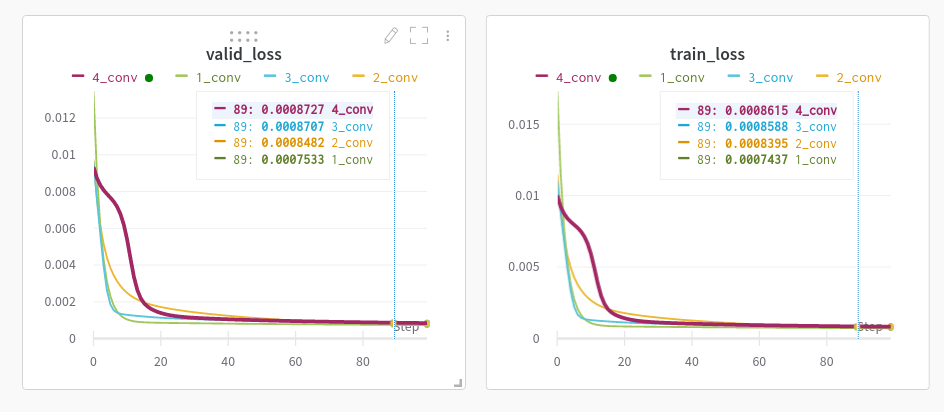
\includegraphics[width=1\textwidth]{figures/conv_layers.png}
        \caption{Effect of Different Conv Layers}
        \label{fig:conv_layers}
    \end{figure}

    \begin{figure}[!htb]
        \centering
        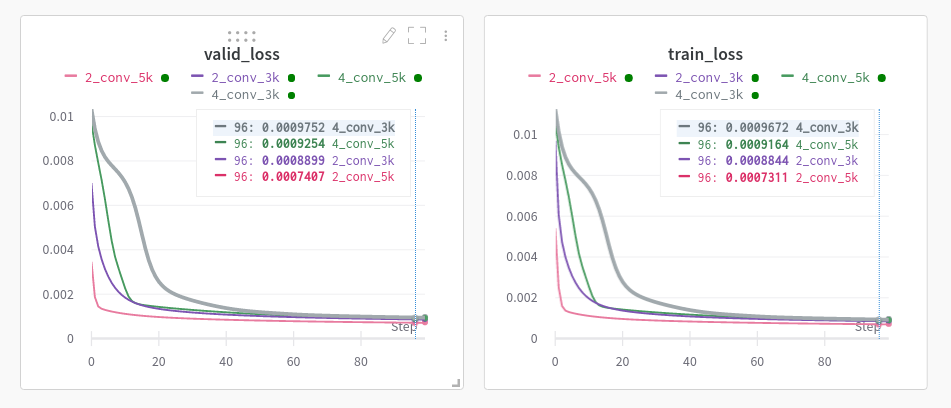
\includegraphics[width=1\textwidth]{figures/conv_kernels.png}
        \caption{Effect of Different Kernel Sizes}
        \label{fig:conv_kernels}
    \end{figure}




\section{Further Experiments (20 pts)}
    Based on your qualitative results (do not forget to give them),
    \begin{itemize}
        \item Try adding a batch-norm layer (torch.nn.BatchNorm2d) into each convolutional layer. How does it affect the results, and, why? Keep it if it is beneficial. 
        \item Try adding a tanh activation function after the very last convolutional layer. How does it affect the results, and, why? Keep it if it is beneficial. 
        
        \item Try setting the number of channels parameter to 16. How does it affect the results, and, why? Keep it if it is beneficial. 
        
      
    \end{itemize}


\section{Your Best Configuration (20 pts)}
Using the best model that you obtain, report the following:
 
    \begin{itemize}
        \item The automatically chosen number of epochs(what was your strategy?):
        \item The plot of the training mean-squared error loss over epochs:
        \item The  plot  of  the  validation  12-margin  error  over  epochs (see the3 text for details):
        \item At least 5 qualitative results on the validation set, showing the prediction and the target colored image:
        \item Discuss the advantages and disadvantages of the model, based on your qualitative results, and, briefly discuss potential ways to improve the model:
    \end{itemize}
    
\section{Your Results on the Test Set(30 pts)}
This part will be obtained by us using the estimations you will provide. Please tell us how should we run your code in case of a problem:

\section{Additional Comments and References}

    (if there any)





\end{document}

